% !TEX TS-program = XeLaTeX
% use the following command:
% all document files must be coded in UTF-8
\documentclass[portuguese]{textolivre}
% build HTML with: make4ht -e build.lua -c textolivre.cfg -x -u article "fn-in,svg,pic-align"

\journalname{Texto Livre}
\thevolume{15}
%\thenumber{1} % old template
\theyear{2022}
\receiveddate{\DTMdisplaydate{2021}{11}{29}{-1}} % YYYY MM DD
\accepteddate{\DTMdisplaydate{2022}{02}{25}{-1}}
\publisheddate{\today}
\corrauthor{Silvani da Silva}
\articledoi{10.35699/1983-3652.2022.37294}
%\articleid{NNNN} % if the article ID is not the last 5 numbers of its DOI, provide it using \articleid{} commmand 
% list of available sesscions in the journal: articles, dossier, reports, essays, reviews, interviews, editorial
\articlesessionname{articles}
\runningauthor{Silva e Ribeiro} 
%\editorname{Leonardo Araújo} % old template
\sectioneditorname{Daniervelin Pereira}
\layouteditorname{Carolina Garcia}

\title{A gestão democrática no Plano de Desenvolvimento Institucional dos Institutos Federais: uma análise a partir do uso do \textit{software} IRaMuTeQ}
\othertitle{Democratic management in the Institutional Development Plan of the Federal Institutes: an analysis based on the use of the IRaMuTeQ software}
% if there is a third language title, add here:
%\othertitle{Artikelvorlage zur Einreichung beim Texto Livre Journal}

\author[1]{Silvani da Silva~\orcid{0000-0003-2207-6965}~\thanks{Email: \url{silvani.silva@ifc.edu.br}}}
\author[1]{Eduardo Augusto Werneck Ribeiro~\orcid{0000-0003-3313-6783}~\thanks{Email: \url{eduardo.ribeiro@ifc.edu.br}}}
\affil[1]{Instituto Federal Catarinense, Mestrado Profissional em Educação Profissional e Tecnológica, Blumenau, SC, Brasil.}

\addbibresource{article.bib}
% use biber instead of bibtex
% $ biber article

% used to create dummy text for the template file
\definecolor{dark-gray}{gray}{0.35} % color used to display dummy texts
\usepackage{lipsum}
\SetLipsumParListSurrounders{\colorlet{oldcolor}{.}\color{dark-gray}}{\color{oldcolor}}

% used here only to provide the XeLaTeX and BibTeX logos
\usepackage{hologo}

% if you use multirows in a table, include the multirow package
\usepackage{multirow}

% provides sidewaysfigure environment
\usepackage{rotating}

% CUSTOM EPIGRAPH - BEGIN 
%%% https://tex.stackexchange.com/questions/193178/specific-epigraph-style
\usepackage{epigraph}
\renewcommand\textflush{flushright}
\makeatletter
\newlength\epitextskip
\pretocmd{\@epitext}{\em}{}{}
\apptocmd{\@epitext}{\em}{}{}
\patchcmd{\epigraph}{\@epitext{#1}\\}{\@epitext{#1}\\[\epitextskip]}{}{}
\makeatother
\setlength\epigraphrule{0pt}
\setlength\epitextskip{0.5ex}
\setlength\epigraphwidth{.7\textwidth}
% CUSTOM EPIGRAPH - END

% LANGUAGE - BEGIN
% ARABIC
% for languages that use special fonts, you must provide the typeface that will be used
% \setotherlanguage{arabic}
% \newfontfamily\arabicfont[Script=Arabic]{Amiri}
% \newfontfamily\arabicfontsf[Script=Arabic]{Amiri}
% \newfontfamily\arabicfonttt[Script=Arabic]{Amiri}
%
% in the article, to add arabic text use: \textlang{arabic}{ ... }
%
% RUSSIAN
% for russian text we also need to define fonts with support for Cyrillic script
% \usepackage{fontspec}
% \setotherlanguage{russian}
% \newfontfamily\cyrillicfont{Times New Roman}
% \newfontfamily\cyrillicfontsf{Times New Roman}[Script=Cyrillic]
% \newfontfamily\cyrillicfonttt{Times New Roman}[Script=Cyrillic]
%
% in the text use \begin{russian} ... \end{russian}
% LANGUAGE - END

% EMOJIS - BEGIN
% to use emoticons in your manuscript
% https://stackoverflow.com/questions/190145/how-to-insert-emoticons-in-latex/57076064
% using font Symbola, which has full support
% the font may be downloaded at:
% https://dn-works.com/ufas/
% add to preamble:
% \newfontfamily\Symbola{Symbola}
% in the text use:
% {\Symbola }
% EMOJIS - END

% LABEL REFERENCE TO DESCRIPTIVE LIST - BEGIN
% reference itens in a descriptive list using their labels instead of numbers
% insert the code below in the preambule:
%\makeatletter
%\let\orgdescriptionlabel\descriptionlabel
%\renewcommand*{\descriptionlabel}[1]{%
%  \let\orglabel\label
%  \let\label\@gobble
%  \phantomsection
%  \edef\@currentlabel{#1\unskip}%
%  \let\label\orglabel
%  \orgdescriptionlabel{#1}%
%}
%\makeatother
%
% in your document, use as illustraded here:
%\begin{description}
%  \item[first\label{itm1}] this is only an example;
%  % ...  add more items
%\end{description}
% LABEL REFERENCE TO DESCRIPTIVE LIST - END


% add line numbers for submission
%\usepackage{lineno}
%\linenumbers

\begin{document}
\maketitle

\begin{polyabstract}
\begin{abstract}
Este trabalho tem como objetivo apresentar uma metodologia inovadora em pesquisa qualitativa utilizada numa pesquisa de pós-graduação em Educação Profissional e Tecnológica. Identificamos a apropriação do termo “gestão democrática” nos Planos de Desenvolvimento Institucionais (PDI) dos Institutos Federais da Rede Federal de Educação Profissional, Científica e Tecnológica do Brasil, a partir de duas premissas: a primeira supõe que em uma instituição criada 20 anos após a Constituição Federal de 1988, o conceito de “gestão democrática” é exercido em sua totalidade e está presente em seu principal documento de planejamento institucional; a segunda é a de que o conceito traz a semântica diretamente relacionada com a dimensão política e pedagógica da gestão escolar, reforçando o tripé ensino, pesquisa e extensão. Tudo isso é resultado de uma instituição educacional comprometida com a formação cidadã e voltada para o mundo do trabalho. Para esta análise, utilizou-se o software IRaMuTeQ como ferramenta de apoio na análise de textos. Avaliou-se, também, a usabilidade da ferramenta para esta tarefa. Este estudo analisou os PDI de 38 Institutos Federais, publicados entre 2014 e 2020 em seus respectivos sites institucionais. A partir das técnicas de Classificação Hierárquica Descendente (CHD), Análise de Similitude e Análise Fatorial por Correspondência (AFC), buscou-se entender como o conceito gestão democrática está materializado e quais são as conexões lexicais nos documentos. Concluiu-se que os PDI são documentos importantes e refletem o entendimento da instituição a cerca do conceito de gestão democrática. As premissas se mostraram parcialmente verdadeiras. Quando foram analisadas as conexões lexicais, o conceito de gestão democrática se mostrou insipiente ou ainda desconectado de outros conceitos com os quais esperava-se dialogar. Esse resultado fomenta a necessidade de novas análises para compreender melhor o fenômeno. Também se confirmou, neste trabalho, o potencial de uso dos recursos técnicos do IRaMuTeQ como ferramenta metodológica em pesquisas qualitativas.

\keywords{Gestão democrática \sep IRaMuTeQ \sep Instituto Federal}
\end{abstract}

\begin{english}
\begin{abstract}
This paper aims to present an innovative methodology in qualitative research used in a postgraduate  investigation in Professional and Technological Education. The appropriation of the term "democratic management" was identified in Institutional Development Plans (IDP) of the Federal Institutes of the Federal Network of Vocational, Scientific and Technological Education in Brazil. It  is based on two premises: the first one assumes that in an institution created 20 years after the 1988 Federal Constitution, the concept of "democratic management" is exercised in its entirety and is present in its main institutional planning document; the second states that the concept brings semantics directly related to the political and pedagogical dimension of school management, reinforcing the tripod teaching, research and extension. This is a result of the proposal of an educational institution committed to  educating for citizenship and to the world of work. For this analysis, the IRaMuTeQ software was used as a support tool in text analysis. We also evaluated the usability of the tool for this task. This study analyzed the IDPs of 38 Federal Institutes, published between 2014 and 2020 on their respective institutional websites. From the techniques of Descending Hierarchical Classification (CHD), Analysis of Similarity, Correspondence Factor Analysis (AFC), we sought to understand how the concept of democratic management is materialized and what the lexical connections are established in the documents. It was concluded that the IDP are important documents and reflect the institution's understanding of the concept of democratic management. The assumptions proved to be partially true. When their lexical connections were analyzed, the concept of democratic management was presented in an incipient way or even disconnected from other concepts that were expected to dialogue. This result encourages new analyses to better understand the phenomenon. This study also confirmed the potential of using the technical resources of IRaMuTeQ as a methodological tool in qualitative research.


\keywords{Democratic management \sep IRaMuTeQ \sep Federal Institute}
\end{abstract}
\end{english}
% if there is another abstract, insert it here using the same scheme
\end{polyabstract}

\section{Introdução}\label{sec-intro}
Este estudo tem como escopo a gestão democrática nos Institutos Federais (IFs). Os IFs são instituições de educação pluricurriculares, com estruturas \textit{multicampi} e apresentam um modelo institucional, especializado na oferta de Educação Profissional e Tecnológica (EPT), em diferentes níveis e modalidades de ensino. Os IFs estão organizados em rede (Rede Federal de Educação Profissional, Científica e Tecnológica – RFEPCT, Lei nº 11.892/2008) \cite{silva_institutos_2009} e foram criados como modelo institucional inovador em relação às demais instituições educacionais brasileiras, por possuírem objetivos específicos que se distinguem tanto das universidades quanto das escolas técnicas tradicionais. A característica \textit{sui generis} pode ser dada pela verticalização do ensino, que possibilita ao aluno cumprir todo seu itinerário formativo na mesma instituição, da educação básica (ensino técnico integrado ao médio) até a pós-graduação (mestrado e doutorado), além de outras modalidades de ensino como educação para jovens e adultos (EJA), cursos subsequentes e de curta duração. Essa característica torna os IFs  instituições educacionais complexas e desafiadoras. Complexas por incorporar, em uma mesma administração, planejamento e gestão da educação básica (ensino médio) e superior. Desafiadoras por trazer consigo premissas legais de que é uma instituição inovadora, comprometido com as exigências de uma educação cidadã, assim, refletindo o contexto histórico de um Estado democrático de direito em que foi criada.

Se considera, neste trabalho, a concepção de gestão democrática voltada para a educação escolar, tendo como entendimento ``[...]a participação considerada como processo inerente à gestão educacional[...]''  \cite[p.~19]{luck_gestao_2006}. A autora também nos apresenta:

\begin{quote}
    O conceito de gestão, portanto, parte do pressuposto de que o êxito de uma organização social depende da mobilização da ação construtiva conjunta de seus componentes, pelo trabalho associado, mediante reciprocidade que cria um “todo” orientado por uma vontade coletiva. Esta, aliás, é condição fundamental para que a educação se processe de forma efetiva no interior da escola, tendo em vista a complexidade e a importância de seus objetivos e processos. \cite[p.~21]{luck_gestao_2006}.
\end{quote}

A autora destaca que a gestão democrática escolar pressupõe em si a ideia de participação, isto é, do trabalho coletivo de pessoas analisando situações, decidindo sobre seu encaminhamento e agindo sobre elas em conjunto.

Considerando essa premissa, diante do conjunto de atribuições e objetivos institucionais dos Institutos Federais, tendo como proposta política e pedagógica a verticalização do ensino, implica refletir sobre a organização administrativa que estes estão construindo. Nesse sentido, o modelo de organização administrativa e de gestão adotado pelos IFs segue diretrizes devidamente referenciadas pela Constituição Federal de 1988, obedecendo princípios como: a) a administração pública, com seus princípios apontados no artigo 37 – Legalidade, Impessoalidade, Moralidade, Publicidade e Eficiência, em que se destaca o tocante à gestão escolar, a publicidade não se restringe apenas à prestação de contas para a sociedade, visa também estimular o interesse e ampliar a comunicação entre a instituição e a comunidade escolar; b) a indissociabilidade entre ensino, pesquisa e extensão, conforme o texto constitucional em seus art. 207, que dispõe também sobre a autonomia didático-científica, administrativa, de gestão financeira e patrimonial das universidades, ressaltando a equiparação dos Institutos Federais \cite{brasil__constituicao_nodate}.

Ainda sobre o modelo de gestão dos IFs, ele atende também aos princípios e fins da educação nacional, estabelecidos pela Lei de Diretrizes e Bases da Educação Nacional (LDB), Lei n° 9394/96 \cite{brasil__lei_nodate} e pela própria Lei nº 11.892 \cite{silva_institutos_2009}. Esse conjunto de normativas, acima de tudo, fundamentam o entendimento que a opção pelo princípio da gestão democrática não é apenas um marco legal, mas também um princípio educativo. Embora os princípios e fins legais estejam consolidados na legislação, é oportuno refletir sobre a avaliação de sua implementação, pois a garantia de sua efetiva execução dependerá do executivo, neste caso, o gestor escolar.

Nesta lógica, a gestão democrática enquanto ação deve sintonizar os preceitos legais com todas as atividades que envolvem uma instituição de educação, considerando a gestão democrática como princípio educativo. \textcite[p.~303]{paro_gestao_1998}, sobre esse aspecto da gestão escolar, diz que o processo educativo tanto as atividades-meio (gestão, assistência ao escolar e atividades complementares) quanto a própria atividade-fim (a relação ensino-aprendizagem que se dá, mas não só) em sala de aula, precisam estar, permanentemente, impregnadas dos fins da educação.

Concorda-se com \textcite{paro_gestao_1998}, pois apesar da existência deste referencial legal sobre a gestão democrática, sem a práxis permanente observando os fins da educação, o conceito pode trazer uma concepção contrária, reforçando o papel da burocratização, que reduz a gestão escolar a uma dimensão tecnicista. Uma gestão democrática, privilegiando as atividades-meio em mediação com as atividades-fim da educação escolar, corroboram não apenas com todas as premissas do autor, como também, atenderá os princípios legais destacados.

Assim como qualquer organização pública, os IFs devem explicitar nos seus documentos norteadores os comprometimentos da instituição com a sociedade, as ações para a consolidação de sua filosofia de trabalho, bem como sua missão, visão, valores, objetivos e metas por um período de cinco anos ou mais. Assim, como se trata de um princípio fundante dos IFs, declaradamente na lei de criação e em seus Estatutos de Criação, o termo “gestão democrática” obrigatoriamente aparece nos Planos de Desenvolvimento Institucionais (PDIs), mas em qual contexto? É o que se procurará discutir neste artigo.

Existem duas premissas que serão avaliadas no artigo. A primeira é que a “gestão democrática” é exercida em sua totalidade, pois nestes 13 anos de experiência de IF, o uso quase obrigatório do termo “gestão democrática” em documentos norteadores, mostram a existência de uma conexão e referência histórica ao compromisso da instituição com os princípios democráticos. Nesta sequência, avaliam-se, dentre os documentos oficiais, os PDIs.

Os PDIs são documentos estratégicos para a gestão e que servem também de base para a formulação dos demais documentos jurídicos constitutivos dessas instituições e têm suas bases na Lei de Diretrizes e Bases da Educação de 1996 e, como os IFs são também considerados instituições de ensino superior, atendem a Lei n.º 10.861 de 14 de abril de 2004, a qual estabeleceu o Sistema Nacional de Avaliação da Educação Superior (Sinaes) \cite{brasil__lei_nodate-1}. Embora já apontado por \textcite{boas_filho_democracia:_2013}, \textcite{lourenco_dos_2019}, \textcite{pogrebinschi_entre_2010}, a existência de polissemia que perpassa o conceito de democracia, supõe-se que o mesmo ocorrerá com o conceito de gestão democrática, uma vez que não são notórios os estudos que possam fundamentar uma análise deste conceito e que procurem apreendê-lo a partir dos PDIs dos IFs. Ressalta-se que as diversas possibilidades dos conceitos gestão democrática e democracia impõe para estes autores, um recorte conceitual para o desenvolvimento deste trabalho. Doravante, explicitamos o conceito adotado.

De modo geral, os PDIs do IF são documentos institucionais construídos coletivamente que objetivam promover os compromissos político e pedagógico a partir de um equilíbrio entre as unidades de gestão (reitoria e os \textit{campi} ou unidades de ensino). Ou seja, apresentam de forma detalhada as responsabilidades e estratégias, visando orientar as ações de suas unidades de ensino para que atinjam os objetivos educacionais.

A segunda premissa a ser avaliada é de ordem teórica. Nos PDIs, a gestão democrática traz a semântica de que o conceito está diretamente relacionado com a dimensão política e pedagógica da gestão escolar, conforme defende \textcite{dourado_gestao_2003}. Esse conceito implica que, ao compartilhar o poder, de certo modo, o mesmo aumenta, pois o verdadeiro poder é compartilhado e não imposto, assim, na coparticipação é que o poder coletivo cresce. Devido à sua complexidade, ao aplicarmos uma metodologia que avalie as ocorrências do termo “gestão democrática" nos PDIs, pode-se identificar qual concepção (semântica) de gestão democrática está explícita ou implícita nestes documentos oficiais (PDIs).

Para isto, aplica-se a proposta metodológica desenvolvida por \textcite{silva_o_2021}, usando o \textit{software} IRaMuTeQ, de código aberto e gratuito, que processa os textos dividindo-os em segmentos denominados unidades de contexto elementar. Neste referido trabalho, a base de dados foram artigos publicados em revistas indexadas (SCOPUS e WoS) cujo os textos relacionam as palavras democracia e escola, cujo o tema abordado foi a escola pública da educação básica e gestão democrática. Estas discussões, em tese, deveriam estar presentes nos PDIs dos Institutos Federais.

No artigo, na seção materiais e métodos, apresenta-se a ferramenta, bem como os parâmetros e indicadores utilizados na análise léxica do termo “gestão democrática" presente nos PDIs de 38 Institutos Federais. Nas seções seguintes (resultados e discussão), descrevem-se a sistematização e a análise dos resultados a partir da fundamentação teórica discutida. Por fim, expõem-se considerações sobre o uso do PDI como fonte de pesquisa para discutir a gestão democrática dentro de uma instituição de educação

\section{Materiais e método}
Esta pesquisa utilizou revisão de literatura para a fundamentação teórica, (artigos científicos) e a utilização de documentos oficiais das instituições para obtenção de dados com fim exploratório-descritivo. Nesse sentido, devido a interpretação que se fará acerca das fontes exploradas, esta pesquisa se caracteriza como pesquisa de natureza básica exploratória, pois busca "uma aproximação com o fenômeno, pelo levantamento de informações que poderão levar o pesquisador a conhecer mais a seu respeito"  \cite[p.~25]{doxsey_metodologia_2002}.

Baseado no algoritmo do ALCESTE, o software IRaMuTeQ, que é um programa computacional de código aberto (gratuito), foi desenvolvido pelo pesquisador francês Pierre \textcite{ratinaud_iramuteq_2014}. Ancorado no \textit{software} estatístico R (\url{www.r-project.org})e na linguagem computacional Python (\url{www.python.org}), o IRaMuTeQ é uma ferramenta de apoio à investigação científica qualitativa que possibilita a organização de grande volume de dados textuais, o gerenciamento e tratamento estatístico de textos, entrevistas ou questionários abertos, otimizando o tempo de análise textual.

Como primeira etapa da pesquisa documental foram baixados pela Internet, os PDIs vigentes, no período de setembro de 2019 a agosto de 2020, diretamente dos \textit{sites} oficiais dessas instituições. Ressalta-se que, para atender o escopo da pesquisa, foram considerados apenas os PDIs dos Institutos Federais de Educação, Ciência e Tecnologia, sendo excluídas outras instituições federais que fazem parte da Rede Federal (RFEPCT), como Colégio Dom Pedro II, os CEFETs, as Escolas Técnicas vinculadas a universidades e á Universidade Tecnológica do Paraná. As instituições excluídas apresentam conformações legais e institucionais anteriores à criação dos IFs. No total foram avaliados 38 PDIs de todos os Institutos Federais em funcionamento no Brasil.

Para avaliar os dados, utilizou-se a combinação de métodos de análise de conteúdo, de acordo com \textcite{bardini_alise_1977} e \textcite{silva_o_2021}. Para \textcite{bardini_alise_1977}, a análise foi desenvolvida em três fases: a pré-análise, a exploração do material e o tratamento dos resultados. Em \textcite{silva_o_2021} é apresentada a operacionalização das etapas supracitadas com a utilização do \textit{software} IRaMuTeQ em todas as fases. É possível acompanhar o processo de desenvolvimento do algoritmo e suas melhorias aplicadas nos estudos de  \textcite{bardini_alise_1977}; \textcite{leblanc_proposition_2016}; \textcite{oliveira_estudo_2003}; \textcite{marchand_quelques_2013}; \textcite{reinert_methode_1983, reinert_logiciel_1986}; \textcite{salem_segments_1986} e \textcite{pelissier_initiation_2017}.

A partir dos PDIs vigentes, foram extraídos dos seus conteúdos somente os textos que tratam da missão, visão e valores institucionais. Foi feita uma leitura no documento para encontrar partes textuais que continham menção ao termo "gestão democrática". Uma vez identificado, o fragmento foi incorporado ao \textit{corpus} textual.

Para cada PDI foi criado um arquivo, atribuído um título iniciando com quatro asteriscos, um espaço e mais um asterisco, nominado em sequência numérica crescente de 1 a 38. Estes foram salvos em uma lista em formato \textit{txt Unicode} (UTF-8), assim formando o \textit{corpus} textual para a análise do conteúdo.

Para a análise de conteúdo, o \textit{software} IRaMuTeQ explorou os conceitos que emergem do \textit{corpus} textual, que é formado pelo conjunto de todos os textos, buscando identificar o sentido léxico que os termos contidos no documento tem, no caso, “gestão democrática”. O algoritmo identifica quais são os conceitos mais importantes que estão em cada arquivo.

Ao proceder à análise do banco de dados, o \textit{software} disponibiliza um relatório estatístico dos textos. Essa informação é apresentada na aba “Resumo” da Análise de texto “Estatística”, que além de mostrar o gráfico de frequência das palavras (\textit{Number of texts}), apresenta outras informações para se avaliar a validade ou não da análise estatística textual feita pelo \textit{software}.

Para a análise de conteúdo, o método aplicado pelo algoritmo foi a léxica automatizada de conteúdos de textos e documentos – Classificação Hierárquica Descendente (CHD). Esse método verifica a correlação entre termos, dentro de um mesmo segmento de texto, que compõem o \textit{corpus} textual, permitindo que se vá além da quantificação de léxicos, passando para uma associação com o contexto em que os termos aparecem. Ressalta-se que a CHD não se caracteriza como uma análise sintática somente, pois possibilita a verificação de como se organizam os termos presentes nos textos e os seus elementos constitutivos.

Por fim, após a aplicação do método CHD, foi possível dispor os resultados na forma de dendrograma, o que permite a organização visual e estatística dos dados. Nesse caso, foi possível visualizar as informações a partir de um dendrograma de distância euclidiana. Ressalta-se que para a disposição do dendrograma foi possível identificar agrupamentos (\textit{cluster}) e a sua ordenação hierárquica descendente, a partir das palavras mais frequentes dentro dos respectivos descritores, considerando cada palavra, a partir de sua importância léxica justificada na análise estatística Qui-quadrado ($\chi^2$). O Teste Qui-quadrado de Independência (não paramétrico) determina se há uma associação entre variáveis categóricas, ou seja, se as variáveis são independentes ou relacionadas.

Ao mostrar a formação de categorias e agrupamentos de classes (\textit{clusters}), foi sistematizada a categorização dos \textit{clusters} pelas palavras-chaves dos PDIs, o que também permitiu visualizar, a partir de um grafo de conexões, o que cada palavra representa no conjunto hierárquico da análise, a partir de suas articulações, formando os entroncamentos léxicos que cada palavra consegue organizar em seus contextos.

\section{Resultado e discussão}
Na análise estatística constatou-se que o total de textos considerados pelo \textit{software} não é o mesmo que o \textit{corpus} textual preparado. Dos 38 arquivos, o \textit{software} apenas considerou 37 documentos. Embora não tenha sido possível identificar os motivos dessa ocorrência, a ausência de um dos textos não trouxe prejuízo à análise, já que, estatisticamente, foi suficiente para que a análise fosse considerada válida com 15.806 palavras (\textit{Number of occurrences}) e 2.043 palavras diferentes (\textit{Number of forms}). Esses quesitos estão de acordo com o estudo realizado por \textcite{silva_o_2021}, onde ficou demonstrado que o algoritmo incorporado ao software realizou a análise do conjunto de textos, constituindo-se um corpus de análise válido.

As \Cref{fig01a} e \Cref{fig01b} mostram duas informações. Em \Cref{fig01a}, estão as classes, e, na \Cref{fig01b}, têm-se as palavras que compõem as classes. Em \Cref{fig01a}, visualiza-se o conjunto de 37 documentos, agrupados em cinco classes ou \textit{clusters}, interligadas por um chaveamento da CHD, que leva em conta as relações entre as palavras no contexto das classes. As linhas dos dendrogramas foram estabelecidas pela distância euclidiana que cada palavra apresentou nos resultados estatísticos. Nesse caso, é possível visualizar, além do número de classes, a participação percentual delas no total de textos. A maior é a classe 5, com 24,8\% dos termos válidos, seguida da classe 4, com 20,8\%; classe 2 com 19,2\%; classe 3 com 18,2\%; e classe 1 com 16,5\%.

Na \Cref{fig01b}, as classes estão denominadas em: Classe 1 – Formação Acadêmica; Classe 2 –Administrativo; Classe 3 – Direitos; Classe 4 – Escola; Classe; e 5 – Institucional. Essa denominação foi organizada a partir do conjunto de palavras que ficaram atribuídas a cada grupo sistematizado pelo software. Nesse sentido, além da similaridade estatística, as palavras-chaves do dendrograma permitiram classificá-las a partir de um recorte analítico que mais sintetizasse a sua reunião.

% \begin{figure}[htbp]
%  \centering
%  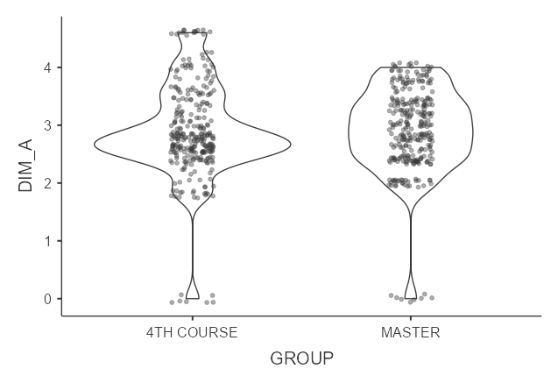
\includegraphics[width=0.85\textwidth]{fig1.eps}
%  \caption{Dendrograma do corpus textual IRaMuTeQ}
%  \label{fig01}
%  \source{Elaborado pelo autor (2021).}
% \end{figure}

% \begin{figure}[htbp]
%  \centering
%  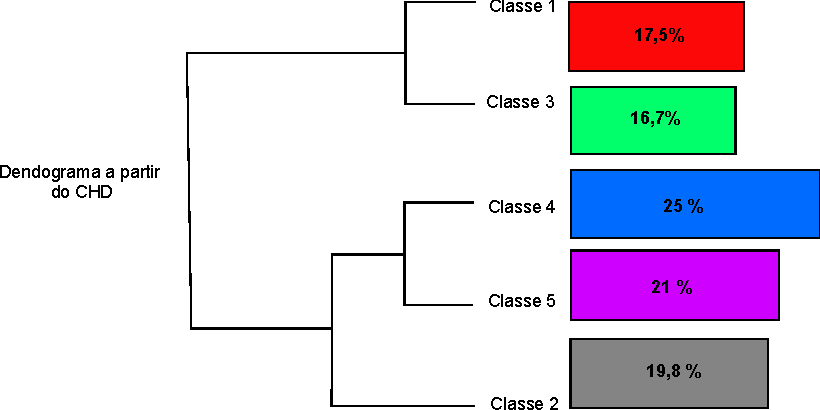
\includegraphics[width=0.85\textwidth]{fig1a.pdf}
%  \caption{Dendrograma do corpus textual IRaMuTeQ (a).}
%  \label{fig01a}
%  \source{Elaborado pelo autor.}
% \end{figure}

% \begin{figure}[htbp]
%  \centering
%  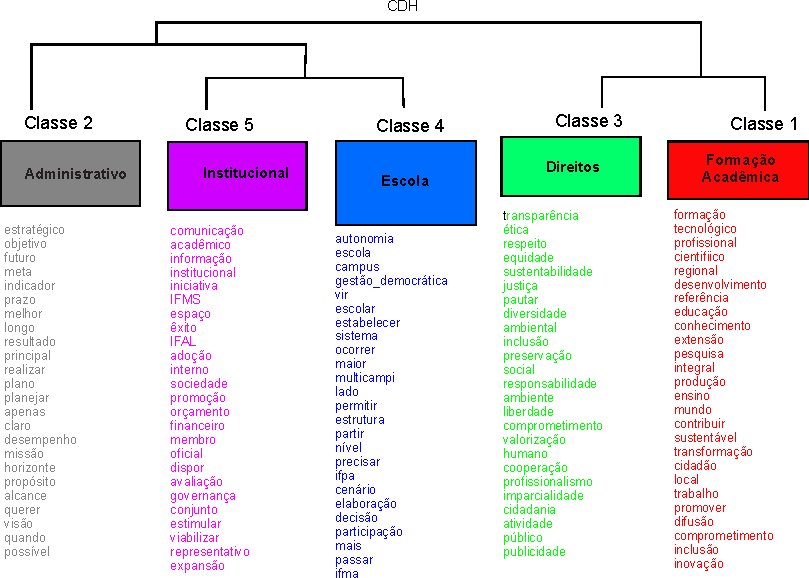
\includegraphics[width=0.85\textwidth]{fig1b.pdf}
%  \caption{Dendrograma do corpus textual IRaMuTeQ (b).}
%  \label{fig01b}
%  \source{Elaborado pelo autor.}
%\end{figure}

\begin{figure}
\centering
\begin{subfigure}[b]{\textwidth}
   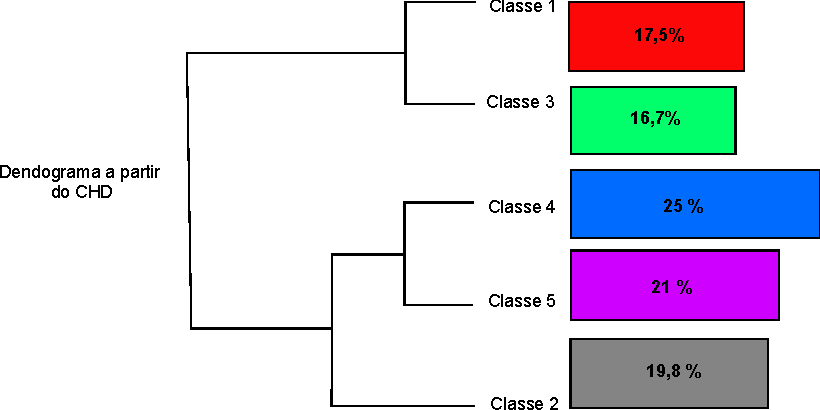
\includegraphics[width=1\linewidth]{fig1a.pdf}
   \caption{}
   \label{fig01a} 
\end{subfigure}
\par\bigskip\par\bigskip
\begin{subfigure}[b]{\textwidth}
   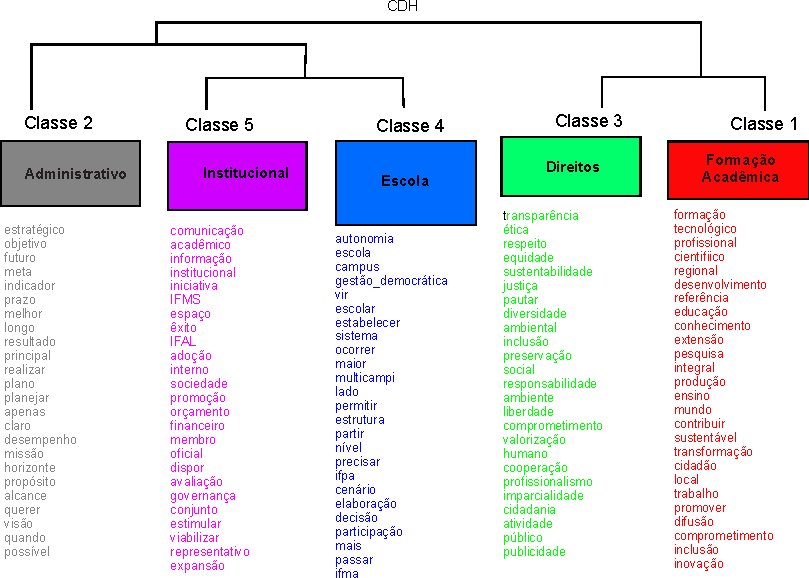
\includegraphics[width=1\linewidth]{fig1b.pdf}
   \caption{}
   \label{fig01b}
\end{subfigure}

\caption{Dendrograma do corpus textual IRaMuTeQ.}
\label{fig01}
\source{Elaborado pelo autor.}
\end{figure}



Destaca-se que a Classificação Hierárquica Descendente (CHD), em forma de dendrograma, é uma importante ferramenta de visualização e análise, pois permite identificar agrupamentos (\textit{cluster}) e a sua ordenação hierárquica descendente, a partir das palavras mais frequentes dentro dos respectivos descritores.

Ao avaliar os agrupamentos representados na \Cref{fig01b}, na apresentação das classes, pode-se evidenciar que a Classe 1 – Formação Acadêmica, ao apresentar palavras como educação, formação, profissional, ensino, pesquisa, extensão, conhecimento, transformação, cidadão, mundo; indica que essa classe reúne o contexto dos objetivos institucionais. Aqui cabe destacar que, pela Lei nº 11.892/2008, os Institutos Federais devem garantir o mínimo de 50\% (cinquenta por cento) de suas vagas para atender a oferta de educação profissional técnica de nível médio \cite{silva_institutos_2009}. Ou seja, a instituição é, eminentemente, uma escola de formação profissional integrada com a educação básica. Essa característica representa um peso importante na balança institucional, no que se refere aos processos de gestão.

Interligada com a Classe 1 – Formação, tem-se a Classe 3 – Direitos, formada por palavras que são termos ligados aos direitos e garantias sociais, tais como transparência, ética, respeito, responsabilidade, justiça, imparcialidade, entre outras, o que denota que, dentro de uma perspectiva da Constituição de 1988, os PDIs garantem o planejamento alinhado aos direitos fundamentais, demonstrando que o ensino essa perspectiva. Entretanto, ao se observar essas palavras posicionadas em colunas diferentes, as similaridades das palavras que caracterizam esses agrupamentos as conectam de acordo com a correlação apresentada nos textos dos PDIs. Observa-se, então que, apesar de conectados, há um relativo distanciamento léxico entre Formação Acadêmica e Direitos das demais classes no chaveamento apresentado pela análise CHD.

Seguindo com os dados da \Cref{fig01b}, as Classes 4 – Escola e Classe e 5 – Institucional apresentam, respectivamente, termos relacionados com autonomia, escola, \textit{campus}, gestão democrática, participação, decisão, bem como comunicação, acadêmico, informação, institucional, espaço, sociedade, entre outras. Ambas as classes se apresentam no dendrograma interligadas, não por acaso, pois as palavras que as compõem representam as condições básicas para que a gestão democrática aconteça. Por estarem em classes separadas, demonstram que, mesmo autônomas, elas estão articuladas entre si.

A palavra autonomia que surge no topo da lista com maior importância na Classe 4 – Escola não é aleatória, a autonomia no contexto da gestão democrática está pautada na concepção de que cada escola tem suas especificidades e, como tal, requer projetos e ações pensadas e elaboradas coletivamente no seu interior por todos os segmentos que a compõem. Sobre a autonomia, \textcite{veiga_escola_2013} a considera como o caminho para a gestão democrática, pois a escola precisa criar mecanismos para garantir a participação da comunidade escolar no processo de organização e gestão dessas instâncias educativas. Nesse aspecto, a gestão democrática, para se materializar, precisa, necessariamente, da autonomia, sendo esta exercida nas discussões e tomadas de decisão coletivas, em que as instâncias decisórias se tornam, também, instâncias educativas de formação política.

Por último, tem-se a Classe 2 – Administrativo, cujas palavras remetem ao espaço voltado ao planejamento institucional, como estratégia, indicador, horizonte, objetivo, meta, futuro, prazo, resultado, entre outras. Considerando a representação das palavras na classe e sua posição no encadeamento com as demais, verifica-se que o espaço Administrativo, de acordo com a análise CHD, representado nos PDIs, está desconectado ou afastado dos demais lugares. Essa constatação é relevante, pois reforça a hipótese que deu origem à pergunta da presente pesquisa, ao apresentar o espaço administrativo, estratégico, desconexo do conjunto que forma a representação discursiva dos PDIs dos Institutos Federais, e mostra-se que é necessário debater sobre a gestão dos IFs, principalmente no que está posto nos PDIs e como isto se reflete na prática, nas diversas instâncias e lugares que compõem essas instituições.

Outro resultado foi a visualização de similaridade das palavras e as conexões que desempenham dentro dos documentos analisados. Conforme a \Cref{fig2}, foi possível utilizar como referência o plano cartesiano, em que os termos estão localizados em uma rede, organizados a partir do termos-chave, ponderados estatisticamente por classes de palavras. Cada palavra gravita (estatisticamente) pela proximidade léxica de outra palavra à qual foi associada. As palavras mais importantes são as que determinam as classes, assim, o nível de ligação entre as palavras indicará a posição na rede.

Tendo como ponto de partida o conhecimento das classes predominantes dadas pela análise representada na \Cref{fig01}, a Análise Fatorial de Correspondência na \Cref{fig2} apresenta uma imagem que agrupa os documentos, cujos discursos são mais congruentes com o assunto pesquisado.

\begin{figure}[htbp]
\centering
\includegraphics[width=0.85\textwidth]{fig2.eps}
\caption{Análise Fatorial de Correspondência dos documentos}
\label{fig2}
\source{Elaborado pelo autor (2021).}
\end{figure}

Nota-se, então, considerando a palavra-chave do tema da pesquisa “gestão democrática” e os seus contextos discursivos que predominam nas Classes 4 e 5, identificadas pela análise CHD com as cores azul e rosa respectivamente, que os documentos mais congruentes estão localizados no Quadrante 1 da \Cref{fig2} e os menos congruentes localizam-se no Quadrante 3.

A interpretação do contexto semântico, a partir dos dados apresentados, podem ser representados a partir da \Cref{fig3}. Nessa imagem, o valor do score do termo é representado a partir da associação das classes, ou seja, a importância lexical representada pelo chi² (X² de associação da palavra com a classe) determina a sua aproximação ou distância da classe principal. Esse resultado da \Cref{fig2} corrobora com a apresentação da \Cref{fig01b}, em que as duas classes 3 e 4 estão interligadas, apresentando uma forte associação, mas mais do que isso, o chi² do termo gestão democrática no gráfico evidencia uma elevada importância dentro da classe.

Outra forma de se visualizar esse resultado são as conexões e suas relações de proximidade (chi²), representadas a partir do conjunto de todas as palavras analisadas nos 38 PDIs, como demonstra a \Cref{fig3}.

\begin{figure}[htbp]
\centering
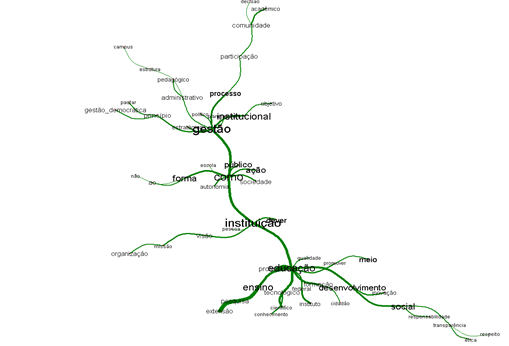
\includegraphics[width=0.85\textwidth]{fig3.png}
\caption{Análise de similitude}
\label{fig3}
\source{Elaborado pelo autor (2021).}
\end{figure}

A \Cref{fig3} se apoia na teoria dos grafos \cite{holanda_notitle_2017}. Trata-se de uma representação gráfica que apresenta uma distribuição das palavras em um plano cartesiano, em que as palavras em comunidades estão distribuídas de acordo com as correlações léxicas entre si, que traduzem o \textit{corpus} textual formado pelos textos dos PDIs analisados.

Por meio da análise de similitude da \Cref{fig3}, foi possível utilizar como referência o plano cartesiano, em que os termos estão localizados em uma rede, organizados a partir do termo-chave, ponderados estatisticamente por classes de palavras. Cada palavra gravita (estatisticamente) pela proximidade léxica de outra palavra à qual foi associada. As palavras mais importantes são as que determinam as classes, assim, o nível de ligação entre as palavras indicará a posição na rede.

A localização da classe gestão democrática na \Cref{fig3} chama a atenção por estar na ponta de uma ramificação, sem nenhuma outra palavra gravitando ou conectada a ela. Em relação com os resultados anteriores apresentados pela CHD (\Cref{fig01}), a gestão democrática está inserida na Classe 4, mas no grafo, o termo mostra-se isolado. O termo desacompanhado apresenta uma possível dicotomia entre teoria (legislação) e a prática (promoção).

%Rever: (\Cref{fig01})

A gestão democrática nas escolas tem seu marco legal inicial com a promulgação da carta magna de 1988, que no texto define a “gestão democrática do ensino público, na forma da lei” como um de seus princípios (Art. 2006, Inciso VI) \cite{brasil__constituicao_nodate}. Em 1996, a LDB determinou em seus artigos 14 e 15, o tocante à gestão democrática, no entanto, essa diretriz não se mostra aplicada, conforme apresentado por \textcite{luck_gestao_2006}, dada a complexidade da efetiva gestão democrática escolar. Embora ainda não consolidada, há que se reconhecer avanços nesse sentido, quando encontramos nos documentos orientadores propostas que reafirmam esta concepção de gestão escolar. Os resultados das análises nos força a concordar com a autora, já que o termo está presente nos documentos, mais claramente inserido no contexto legal e distante do contexto das práticas educativas.

Esperava-se que esta concepção de gestão voltada para a educação escolar deveria ter em sua ramificação, palavras que indicassem a participação, o conselho ou mesmo a palavra representações como demonstram os estudos de \textcite{fernandes_construcao_2009} e \textcite{souza_o_2018}.

A expectativa de que o conceito de gestão democrática nos PDIs, 20 anos após a Constituição Federal, estivesse mais explícito e consolidado, não se realizou. A promoção da participação da comunidade, por meio de seus representantes, como demonstram  \textcite{diniz_junior_os_2019}, na tomada de decisão é entendida como apenas um dos vários procedimentos administrativos que, mesmo que considerados como democráticos (a exemplo de estruturas como conselhos, colegiados e eleições para gestores) deveriam estar mais próximos a outros grupos de palavras ou mesmo seria desejável que suas conexões estivessem mais evidentes. O resultado da análise dos 38 documentos, com separação a partir das conexões apresentadas na \Cref{fig3}, bem como a forma em que as palavras foram agrupadas, mostraram que esta observação não é um caso particular.

Portanto, apesar de apresentar-se com estruturas participativas em forma de conselhos e colegiados, com procedimentos considerados democráticos, como eleições para os cargos de gestão, não se pode garantir que essas instâncias administrativas sejam suficientes para que, de fato, se caracterize a gestão democrática. De acordo com \textcite{souza_as_2019}, essas estruturas contribuem ou potencializam para a gestão democrática, mas não são capazes de edificá-la, por si só. Nesse mesmo sentido, dentro dos limites que uma pesquisa como esta apresenta, considerando somente análise léxica dos textos dos documentos, é possível visualizar também na \Cref{fig3}, uma significativa distância entre o termo gestão democrática e as demais palavras que representam a Classe Escola e a Classe Formação. Ambas estão em posições extremamente opostas na \Cref{fig3}, ensejando que no discurso textual dos PDIs dos Institutos Federais, as atividades-fim não acompanham a gestão democrática de acordo com o conceito referenciado nos próprios documentos.

Mesmo que exista a pretensão em palavras (no caso, dos PDIs), nos Institutos Federais, em adotar o princípio da gestão democrática, tendo como referência o conceito de gestão democrática e educação definido por \textcite{freire_educacao_1983,freire_professora_1993,freire_pedagogia_2000}, \textcite{luck_gestao_2006}, \textcite{paro_gestao_1998}, \textcite{veiga_escola_2013}, entre outros autores consagrados no campo da educação progressista, é necessário avaliar seus próprios discursos nos PDIs, em relação às intenções e práticas realizadas ou não. Assim, os contextos da Classe Escola e Classe Formação Acadêmica, conforme expostos pela análise lexical nos PDIs, para que se materialize na prática, precisam estar, além de politico e pedagogicamente, textualmente conectados, ou seja, precisam estar no mesmo contexto, pois a gestão democrática é e deve ser, também, um processo de formação permanente.

Percebeu-se que nos textos dos PDIs, a organização dos espaços educativos da EPT, no que se refere esta pesquisa, a classe gestão democrática está distante e sem diálogo entre a Classe Escola e a Classe Formação Acadêmica. Constatação que está longe do que pensou \textcite{paro_gestao_1998} quando defendeu o princípio educativo incutido na gestão escolar, diz que o processo educativo tanto as atividades-meio (gestão, assistência ao escolar e atividades complementares) quanto a própria atividade-fim (a relação ensino-aprendizagem que se dá, mas não só) em sala de aula, precisam estar, permanentemente, impregnadas dos fins da educação. Considerando o pensamento de \textcite{paro_gestao_1998}, diante dos textos analisados, é possível afirmar que não há evidências que os PDIs indiquem claramente e de forma destacada uma proposta de formação cidadã e democrática com participação efetiva em todos os espaços pedagógicos. Esperava-se que, por serem instituições criadas 20 anos após a Constituição Federal, o princípio da gestão democrática deveria estar mais explícito no PDI.

Desse modo, os PDIs precisam promover a gestão democrática nos textos, de maneira mais explícita, detalhada e refletida, pois o conceito de gestão escolar, aqui entendido, pressupõe a participação efetiva de todos os segmentos da comunidade escolar, pais, professores, estudantes e funcionários.

Portanto, a gestão democrática deve ser entendida como um processo de formação permanente, tanto nos espaços formais de educação, que se referem às mais diferentes etapas e áreas da gestão escolar (planejamento, implementação e avaliação), como na construção dos projetos e processos pedagógicos, que também envolvem os espaços não formais, ligados a participação da comunidade, fora da estrutura burocratizada da instituição.

Tanto \textcite{paro_gestao_1998}, \textcite{dourado_gestao_2003} e \textcite{luck_gestao_2006}, já citados, como também \textcite{boas_filho_democracia:_2013}, \textcite{lourenco_dos_2019} e \textcite{pogrebinschi_entre_2010}, ao alertarem que o conceito de democracia deveria também ser aplicado ao conceito de gestão democrática, o que se mostrou é que os PDIs dos IFs ainda não avançaram em apreendê-lo. Essa constatação, por sua vez, pode esvaziar a formação ou transformação da cultura institucional, baseada no diálogo igualitário, na horizontalidade e corresponsabilidade entre as diferentes forças que compõem essas instituições.

\section{Considerações finais}\label{sec-organizacao}
A partir do conceito de gestão democrática, foi possível discutir as duas premissas do trabalho. A primeira é de que a “gestão democrática”, exercida em sua totalidade, se mostrou ainda no campo das intenções, indo, em alguns aspectos, na contramão do que foi estudado em relação à gestão democrática. Ou seja, ao constatar-se que nos PDIs analisados o termo gestão democrática não aparece em todas as partes/classes avaliadas, confirmando-se assim o que os autores que discutem o tema e defendem a efetiva execução da gestão democrática escolar é uma proposta onde existe a participação e o entendimento de que o espaço deve ser gerido com diálogo e planejamento coletivo. Que apesar dos avanços dos colegiados, da construção dos PDIS e PPPs, eleição de diretores, Conselhos, entre outros previstos na legislação, ainda há muito que se avançar tanto na gestão das unidades de ensino, quanto no fazer pedagógico em criar espaços de vivência da participação, da decisão, da cidadania plena.

A segunda, por meio das análises realizadas com a ajuda do \textit{software} IRaMuTeQ, percebeu-se que, nos textos dos PDIs, as palavras que compõem as classes da organização dos espaços educativos, no que se refere à pesquisa, ao ensino, à extensão e à gestão, bem como no planejamento, a Classe Gestão Democrática está distante e sem diálogo com a Classe Escola e a Classe Formação Acadêmica. Apresentando-se de forma incipiente em muitos desses documentos, o que incentiva novas análises para compreender melhor esse fenômeno.

Concluímos com esse estudo que os PDIs não contemplam as duas premissas que abordamos nesse artigo. Finalizamos afirmando que estes documentos devem refletir todos os espaços institucionais, principalmente no espaço formativo basilar de qualquer organização, as relações humanas presentes nos espaços formais e não formais, o que fomenta a construção e a apropriação do conceito em seu puro exercício.

Desta forma, a gestão democrática deve ser entendida como um processo de formação permanente, tanto nos espaços formais e informais, nas mais diferentes etapas e áreas da gestão escolar. Assim poderemos ampliar as experiências no planejamento, implementação e avaliação, bem como na construção dos projetos e processos pedagógicos com a sociedade, possibilitando o exercício da participação da comunidade na aplicação dos importantes conceitos aqui discutidos.



\printbibliography\label{sec-bib}
% if the text is not in Portuguese, it might be necessary to use the code below instead to print the correct ABNT abbreviations [s.n.], [s.l.]
%\begin{portuguese}
%\printbibliography[title={Bibliography}]
%\end{portuguese}


%full list: conceptualization,datacuration,formalanalysis,funding,investigation,methodology,projadm,resources,software,supervision,validation,visualization,writing,review
\begin{contributors}[sec-contributors]
\authorcontribution{Silvani da Silva}[conceptualization, writing, methodology, software]
\authorcontribution{Eduardo A. W. Ribeiro}[writing,review]
\end{contributors}





\end{document}

